\chapter{Monte Carlo Simulation}\label{cap:montecarlo}

The modern version of the Monte Carlo method dates back to the
introduction of the first computers and their application during the
years 1940-45 with the purpose of computing neutron diffusion in atomic
bombs.

The Monte Carlo approach was primarily promoted by physics
researchers Stanislaw Ulam, Nicholas Metropolis and John von Neumann.
They were well aware of the potential of such techniques but it was only
with the first electronic computer - the ENIAC - which was able to solve
differential equations at a tremendous, so far unconceivable speed, the
Monte Carlo method was eventually triggered.

The name Monte Carlo refers to a famous casino in Monaco where Ulam's
uncle used to indulge his gambling passion. 
The characteristics of
randomness and the repetitive nature of many processes correspond with
the games played in a casino. Note that the famous roulette wheel is
one of the simplest mechanical devices to generate random variables.

Simulation tools find their application mostly in cases where the
inherent complexity of a problem makes the use of other techniques
impossible or where no analytically tractable solution with a
deterministic algorithm is existing. In short, \emph{the Monte Carlo method is
a numerical approach which aims for solving mathematical problems by the
simulation of random variables}.

Monte Carlo simulations are widely used in many fields: Engineering,
Physics, Computational biology, Computer graphics, Applied statistics and 
Artificial intelligence for games.

It started to be en vogue in financial mathematics in the 1980s,
particularly when the theories of the random walk of asset prices came
up.

%The modern version of the Monte Carlo method was invented in the late
%1940s by Stanislaw Ulam, while he was working on nuclear weapon
%projects at the Los Alamos National Laboratory.

%Monte Carlo methods, or experiments, are a broad class of computational
%algorithms that rely on repeated random sampling to obtain numerical
%results; the underlying concept is to use randomness to solve problems
%that might be deterministic in principle. Monte Carlo methods are mainly
%used in three problem classes: optimization, numerical integration, and
%generating draws from a probability distribution.

In this Chapter this very important technique is reviewed and presented
beside some useful applications.

\section{The Algorithm}\label{whats-monte-carlo-simulation}

Monte Carlo (MC) methods are used when a closed-form solution for a
property being studied cannot be developed.

A MC simulation performs analysis by building a model and producing 
results from it by substituting, for any factor that has inherent uncertainty,
the PDF of the corresponding random variable. 
Model results are calculated over and over, each time using a different set of
random values from the aforementioned probability distributions. 
Depending upon the number of uncertainties and the ranges specified for them,
a Monte Carlo simulation could involve thousands or even millions of
calculations before it is completed. Finally the simulation produces the
distribution of possible outcome values.

A MC method/algorithm then can be described as follows: 
\begin{itemize}
	\item  select a domain \(\Omega\) for the inputs (probability distributions for our factors); 
	\item generate random inputs from this domain \(\Omega\);
	\item perform a deterministic computation with those inputs;
	\item aggregate the results.
\end{itemize}

In the next Sections we will see each step in the implementation of
practical examples.

\section{Pseudo-Random Numbers}
\label{pseudo-random-numbers}

The need of generating random inputs during a MC simulation requires 
large amounts of \emph{random numbers} to be generated, and it was their use
that spurred the development of pseudo-random number generators. 

Nowadays every programming language has libraries that allows to produce 
huge series of random numbers (with a periodicity of \(2^{19937}\)). These
series are calculated by algorithms that take as input a \emph{seed} which
determines them uniquely. This means that choosing the same seed you will
produce the same set of numbers every time (which is great for debugging
purposes).

In \texttt{python} one of the available modules to generate random numbers is \texttt{random} which has, among others, the following useful functions:
\begin{itemize}
\tightlist
\item
  \texttt{seed}: set the seed of the random number generator;
\item
  \texttt{random}: returns a random number between 0 and 1 (with uniform
  probability);
\item
  \texttt{randint(min,\ max)}: returns an integer random number between
  \texttt{min} and \texttt{max} (with uniform probability);
\item
  \texttt{sample(aList,\ k=n)}: samples n elements from the list
  \texttt{aList}.
\end{itemize}
\noindent
As usual for a more detailed description check \texttt{help(random)}.

The following example shows an application of these functions beside the effect of  changing the random number generator seed.

\begin{codebox}[breakable, size=fbox, boxrule=1pt, pad at break*=1mm,colback=cellbackground, colframe=cellborder]
\begin{Verbatim}[commandchars=\\\{\}]
\PY{k+kn}{import} \PY{n+nn}{random} 

\PY{n}{random}\PY{o}{.}\PY{n}{seed}\PY{p}{(}\PY{l+m+mi}{1}\PY{p}{)}
\PY{n+nb}{print} \PY{p}{(}\PY{l+s+s2}{\PYZdq{}}\PY{l+s+s2}{seed is 1}\PY{l+s+s2}{\PYZdq{}}\PY{p}{)}
\PY{n+nb}{print}\PY{p}{(}\PY{n}{random}\PY{o}{.}\PY{n}{random}\PY{p}{(}\PY{p}{)}\PY{p}{)}
\PY{n+nb}{print}\PY{p}{(}\PY{n}{random}\PY{o}{.}\PY{n}{random}\PY{p}{(}\PY{p}{)}\PY{p}{)}

\PY{n}{random}\PY{o}{.}\PY{n}{seed}\PY{p}{(}\PY{l+m+mi}{2}\PY{p}{)}
\PY{n+nb}{print} \PY{p}{(}\PY{l+s+s2}{\PYZdq{}}\PY{l+s+s2}{seed is 2}\PY{l+s+s2}{\PYZdq{}}\PY{p}{)}
\PY{n+nb}{print}\PY{p}{(}\PY{n}{random}\PY{o}{.}\PY{n}{random}\PY{p}{(}\PY{p}{)}\PY{p}{)}
\PY{n+nb}{print}\PY{p}{(}\PY{n}{random}\PY{o}{.}\PY{n}{random}\PY{p}{(}\PY{p}{)}\PY{p}{)}

\PY{n}{random}\PY{o}{.}\PY{n}{seed}\PY{p}{(}\PY{l+m+mi}{1}\PY{p}{)}
\PY{n+nb}{print} \PY{p}{(}\PY{l+s+s2}{\PYZdq{}}\PY{l+s+s2}{seed is 1 again}\PY{l+s+s2}{\PYZdq{}}\PY{p}{)}
\PY{n+nb}{print}\PY{p}{(}\PY{n}{random}\PY{o}{.}\PY{n}{random}\PY{p}{(}\PY{p}{)}\PY{p}{)}
\PY{n+nb}{print}\PY{p}{(}\PY{n}{random}\PY{o}{.}\PY{n}{random}\PY{p}{(}\PY{p}{)}\PY{p}{)}

\PY{n+nb}{print}\PY{p}{(}\PY{n}{random}\PY{o}{.}\PY{n}{randint}\PY{p}{(}\PY{l+m+mi}{1}\PY{p}{,} \PY{l+m+mi}{10}\PY{p}{)}\PY{p}{)}
\PY{n}{aList} \PY{o}{=} \PY{p}{[}\PY{l+s+s1}{\PYZsq{}}\PY{l+s+s1}{a}\PY{l+s+s1}{\PYZsq{}}\PY{p}{,} \PY{l+s+s1}{\PYZsq{}}\PY{l+s+s1}{b}\PY{l+s+s1}{\PYZsq{}}\PY{p}{,} \PY{l+s+s1}{\PYZsq{}}\PY{l+s+s1}{c}\PY{l+s+s1}{\PYZsq{}}\PY{p}{,} \PY{l+s+s1}{\PYZsq{}}\PY{l+s+s1}{d}\PY{l+s+s1}{\PYZsq{}}\PY{p}{,} \PY{l+s+s1}{\PYZsq{}}\PY{l+s+s1}{f}\PY{l+s+s1}{\PYZsq{}}\PY{p}{]}
\PY{n+nb}{print} \PY{p}{(}\PY{n}{random}\PY{o}{.}\PY{n}{sample}\PY{p}{(}\PY{n}{aList}\PY{p}{,} \PY{n}{k}\PY{o}{=}\PY{l+m+mi}{2}\PY{p}{)}\PY{p}{)}

seed is 1
0.13436424411240122
0.8474337369372327
seed is 2
0.9560342718892494
0.9478274870593494
seed is 1 again
0.13436424411240122
0.8474337369372327
2
['c', 'a']
\end{Verbatim}
\end{codebox}

The next lines of code show instead how to draw a uniform distribution. Figure~\ref{fig:uniform_dist} shows the result.

 \begin{codebox}[breakable, size=fbox, boxrule=1pt, pad at break*=1mm,colback=cellbackground, colframe=cellborder]
\begin{Verbatim}[commandchars=\\\{\}]
\PY{n}{numbers} \PY{o}{=} \PY{p}{[}\PY{p}{]}
\PY{k}{for} \PY{n}{\PYZus{}} \PY{o+ow}{in} \PY{n+nb}{range}\PY{p}{(}\PY{l+m+mi}{10000}\PY{p}{)}\PY{p}{:}
  \PY{n}{numbers}\PY{o}{.}\PY{n}{append}\PY{p}{(}\PY{n}{random}\PY{o}{.}\PY{n}{randint}\PY{p}{(}\PY{l+m+mi}{0}\PY{p}{,} \PY{l+m+mi}{5}\PY{p}{)}\PY{p}{)}

\PY{k+kn}{from} \PY{n+nn}{matplotlib} \PY{k}{import} \PY{n}{pyplot} \PY{k}{as} \PY{n}{plt}
\PY{n}{plt}\PY{o}{.}\PY{n}{hist}\PY{p}{(}\PY{n}{numbers}\PY{p}{,} \PY{l+m+mi}{6}\PY{p}{,} \PY{n+nb}{range}\PY{o}{=}\PY{p}{[}\PY{o}{\PYZhy{}}\PY{l+m+mf}{0.5}\PY{p}{,} \PY{l+m+mf}{5.5}\PY{p}{]}\PY{p}{)}
\PY{n}{plt}\PY{o}{.}\PY{n}{title}\PY{p}{(}\PY{l+s+s2}{\PYZdq{}}\PY{l+s+s2}{Uniform distribution from randint}\PY{l+s+s2}{\PYZdq{}}\PY{p}{)}
\PY{n}{plt}\PY{o}{.}\PY{n}{show}\PY{p}{(}\PY{p}{)}
\end{Verbatim}
\end{codebox}

\begin{figure}[h]
\centering
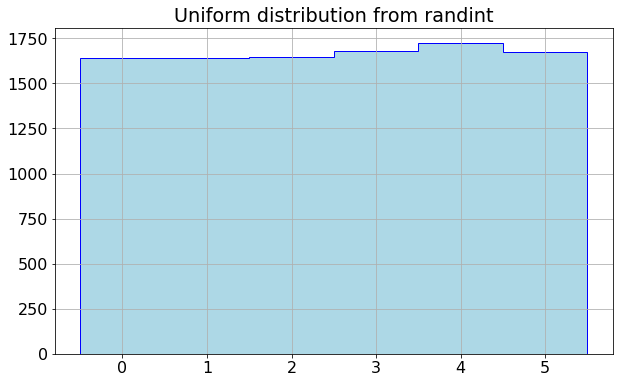
\includegraphics[width=0.7\textwidth]{figures/uniform.png}
\caption{Uniform distribution generated with \texttt{random.randint} function.}
\label{fig:uniform_dist}
\end{figure}
    
Another useful module that is used later to generate random numbers is \texttt{numpy}. It has similar functionalities to \texttt{random} but in some cases it fits better to our needs.    
Below an example with \texttt{numpy.random.normal} which allows to throw random numbers according to a normal distribution
(\(\mathcal{N}(0, 1)\)), its plot is shown in Fig.~\ref{fig:gauss_dist}.

\begin{codebox}[breakable, size=fbox, boxrule=1pt, pad at break*=1mm,colback=cellbackground, colframe=cellborder]
\begin{Verbatim}[commandchars=\\\{\}]
\PY{k+kn}{from} \PY{n+nn}{numpy}\PY{n+nn}{.}\PY{n+nn}{random} \PY{k}{import} \PY{n}{normal}
\PY{k+kn}{from} \PY{n+nn}{matplotlib} \PY{k}{import} \PY{n}{pyplot} \PY{k}{as} \PY{n}{plt}

\PY{n}{gauss} \PY{o}{=} \PY{p}{[}\PY{p}{]}
\PY{k}{for} \PY{n}{\PYZus{}} \PY{o+ow}{in} \PY{n+nb}{range}\PY{p}{(}\PY{l+m+mi}{50000}\PY{p}{)}\PY{p}{:}
  \PY{n}{gauss}\PY{o}{.}\PY{n}{append}\PY{p}{(}\PY{n}{normal}\PY{p}{(}\PY{p}{)}\PY{p}{)}
  
\PY{n}{plt}\PY{o}{.}\PY{n}{hist}\PY{p}{(}\PY{n}{gauss}\PY{p}{,} \PY{l+m+mi}{100}\PY{p}{,} \PY{n+nb}{range}\PY{o}{=}\PY{p}{[}\PY{o}{\PYZhy{}}\PY{l+m+mi}{4}\PY{p}{,} \PY{l+m+mi}{4}\PY{p}{]}\PY{p}{)}
\PY{n}{plt}\PY{o}{.}\PY{n}{title}\PY{p}{(}\PY{l+s+s2}{\PYZdq{}}\PY{l+s+s2}{Example of Gaussian distribution from numpy}\PY{l+s+s2}{\PYZdq{}}\PY{p}{)}
\PY{n}{plt}\PY{o}{.}\PY{n}{show}\PY{p}{(}\PY{p}{)}
\end{Verbatim}
\end{codebox}

 \begin{figure}
   \centering
   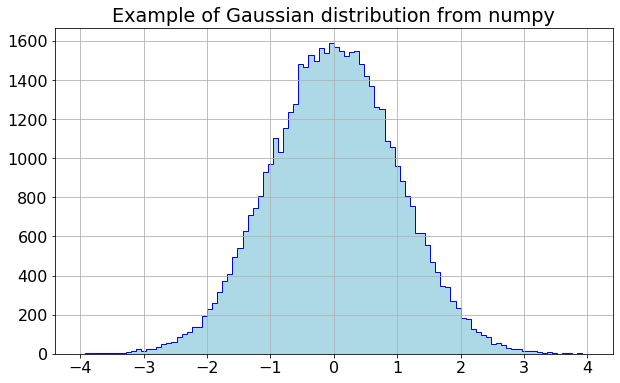
\includegraphics[width=0.7\textwidth]{figures/standard_normal}
   \caption{Normal distribution generated with \texttt{numpy.random.normal} function.}
\label{fig:gauss_dist}
 \end{figure}

%\hypertarget{acceptance-rejection-method}{%
%\subsubsection{Acceptance-Rejection
%	Method}\label{acceptance-rejection-method}}
%
%The acceptance-rejection method was proposed by von Neumann in 1951 and
%is used in order to generate random variables that follow a probability
%density function denoted by \(f(x)\). Since we are occasionally
%struggling in inverting the CDF that corresponds to our \(f(x)\), the
%just discussed inverse transform method loses ground and the
%acceptance-rejection method is applied.
%
%Given a so called target distribution \(f(x)\), the acceptance-rejection
%method generates samples according to \(f(x)\) by first of all
%generating samples from a more suitable distribution \(g(y)\).
%Afterwards a random subset of these generated samples is rejected
%according to certain rejection rules. Thereby the choice of this
%rejection rule, or let us call it rejection approach, will be decisive
%if the accepted samples will eventually be distributed according to
%\(f(x)\). The property \(f(x) \leq c\cdot g(x)\), for some constant
%\(c\), tells us now how to generate samples from \(g(y)\). Therefore, we
%conclude that in the acceptance-rejection method a sample \(Y\) is
%generated from \(g\) and at the same time accepted with probability
%\(f(Y)/cg(Y)\). The generic implementation, i.e.~the algorithm of the
%acceptance-rejection method that we can use to sample from density \(f\)
%using candidates from \(g\), can be stated as follows:
%
%\begin{enumerate}
%\def\labelenumi{\arabic{enumi}.}
%\tightlist
%\item
%generate the sample \(Y\) from the distribution with density \(g\)
%\item
%generate \(u\) from \(U[0,1]\), which must be independent of \(Y\)
%\item
%if \(u\leq f(Y)/cg(Y)\), then deliver \(X = Y\), otherwise return to
%step 1.
%\end{enumerate}

\section{Practical Examples of Monte Carlo
Simulation}\label{example-of-monte-carlo-simulation}

In this Section we go through some applications of the Monte Carlo method.

\subsection{Probability to draw two kings from a deck}
Using a frequentist approach, we can calculate the
probability of an event as the ratio of the number of favorable outcomes
of an experiment (number of successes) and the number of all possible
outcomes. 

Imagine we would like to determine the probability of drawing two kings from a standard deck of cards.
At the beginning we have 40 cards (i.e. the entire deck) with 4 possible kings so the probability to get a king is $4/40$. Next, assuming we got a king the first time, we are left with 39 cards and 3 kings only so the probability to get the second king is $3/39$. Since we want both events to happen, the final probability is the product of the two contributions:

\begin{equation*}
P_\textrm{two kings} = \frac{4}{40} \cdot \frac{3}{39} = \frac{1}{130} \approx 0.0077
\end{equation*}

Let's now try to estimate the same probability with a MC simulation, following
the steps outlined above, and check if we get the same number.
\begin{itemize}
\item \emph{Define a domain of possible inputs}: in this case the domain is a deck of cards. So a list with all the possible cards is defined (with the multiplicative operator (\texttt{*}) a list can be repeated many times; in this case, four times once for each suit). The seed is also set to 1 to make the
test reproducible.

\begin{codebox}[breakable, size=fbox, boxrule=1pt, pad at break*=1mm,colback=cellbackground, colframe=cellborder]
\begin{Verbatim}[commandchars=\\\{\}]
\PY{k+kn}{from} \PY{n+nn}{random} \PY{k}{import} \PY{n}{sample}\PY{p}{,} \PY{n}{choices}\PY{p}{,} \PY{n}{seed}

\PY{n}{seed}\PY{p}{(}\PY{l+m+mi}{1}\PY{p}{)}
\PY{n}{deck} \PY{o}{=} \PY{p}{[}\PY{l+s+s2}{\PYZdq{}}\PY{l+s+s2}{A}\PY{l+s+s2}{\PYZdq{}}\PY{p}{,} \PY{l+s+s2}{\PYZdq{}}\PY{l+s+s2}{2}\PY{l+s+s2}{\PYZdq{}}\PY{p}{,} \PY{l+s+s2}{\PYZdq{}}\PY{l+s+s2}{3}\PY{l+s+s2}{\PYZdq{}}\PY{p}{,} \PY{l+s+s2}{\PYZdq{}}\PY{l+s+s2}{4}\PY{l+s+s2}{\PYZdq{}}\PY{p}{,} \PY{l+s+s2}{\PYZdq{}}\PY{l+s+s2}{5}\PY{l+s+s2}{\PYZdq{}}\PY{p}{,} \PY{l+s+s2}{\PYZdq{}}\PY{l+s+s2}{6}\PY{l+s+s2}{\PYZdq{}}\PY{p}{,} \PY{l+s+s2}{\PYZdq{}}\PY{l+s+s2}{7}\PY{l+s+s2}{\PYZdq{}}\PY{p}{,} \PY{l+s+s2}{\PYZdq{}}\PY{l+s+s2}{J}\PY{l+s+s2}{\PYZdq{}}\PY{p}{,} \PY{l+s+s2}{\PYZdq{}}\PY{l+s+s2}{Q}\PY{l+s+s2}{\PYZdq{}}\PY{p}{,} \PY{l+s+s2}{\PYZdq{}}\PY{l+s+s2}{K}\PY{l+s+s2}{\PYZdq{}}\PY{p}{]} \PY{o}{*} \PY{l+m+mi}{4}
 \end{Verbatim}
\end{codebox}

\item \emph{Generate inputs randomly from a probability distribution over the defined domain}: which means we draw randomly cards with uniform probability since the deck is fair (all cards have the same probability to be drawn). 
We plan to do 1 million simulations; each time with the \texttt{sample} function we pick up two cards from our virtual deck (for debugging purpose the first 10 trials are printed).

\begin{codebox}[breakable, size=fbox, boxrule=1pt, pad at break*=1mm,colback=cellbackground, colframe=cellborder]
\begin{Verbatim}[commandchars=\\\{\}]
\PY{n}{trials} \PY{o}{=} \PY{l+m+mi}{1000000}
\PY{n}{successes} \PY{o}{=} \PY{l+m+mi}{0}

\PY{k}{for} \PY{n}{i} \PY{o+ow}{in} \PY{n+nb}{range}\PY{p}{(}\PY{n}{trials}\PY{p}{)}\PY{p}{:}
  \PY{n}{cards} \PY{o}{=} \PY{n}{sample}\PY{p}{(}\PY{n}{deck}\PY{p}{,} \PY{n}{k}\PY{o}{=}\PY{l+m+mi}{2}\PY{p}{)}
  \PY{k}{if} \PY{n}{i} \PY{o}{\PYZlt{}} \PY{l+m+mi}{10}\PY{p}{:}
    \PY{n+nb}{print} \PY{p}{(}\PY{n}{cards}\PY{p}{)}
\end{Verbatim}
\end{codebox}

\item \emph{Perform a deterministic computation on the generated inputs}: this step is particularly simple in this case, we just need to check if the draw is \texttt{['K', 'K']} and in case increase the counter of successes.

\begin{codebox}[breakable, size=fbox, boxrule=1pt, pad at break*=1mm,colback=cellbackground, colframe=cellborder]
\begin{Verbatim}[commandchars=\\\{\}]
  \PY{k}{if} \PY{n}{cards} \PY{o}{==} \PY{p}{[}\PY{l+s+s2}{\PYZdq{}}\PY{l+s+s2}{K}\PY{l+s+s2}{\PYZdq{}}\PY{p}{,} \PY{l+s+s2}{\PYZdq{}}\PY{l+s+s2}{K}\PY{l+s+s2}{\PYZdq{}}\PY{p}{]}\PY{p}{:}
    \PY{n}{successes} \PY{o}{+}\PY{o}{=} \PY{l+m+mi}{1}
 \end{Verbatim}
\end{codebox}

\item \emph{Aggregate the results}: finally we just print successes/trials which is the sought probability.

\begin{codebox}[breakable, size=fbox, boxrule=1pt, pad at break*=1mm,colback=cellbackground, colframe=cellborder]
\begin{Verbatim}[commandchars=\\\{\}]
\PY{n+nb}{print} \PY{p}{(}\PY{l+s+s2}{\PYZdq{}}\PY{l+s+s2}{The probability to draw two kings is }\PY{l+s+si}{\PYZob{}:.4f\PYZcb{}}\PY{l+s+s2}{\PYZdq{}}\PY{o}{.}\PY{n}{format}\PY{p}{(}\PY{n}{successes}\PY{o}{/}\PY{n}{trials}\PY{p}{)}\PY{p}{)}

['Q', '7']
['5', '7']
['J', '2']
['Q', 'A']
['5', '4']
['7', '2']
['2', '5']
['J', 'Q']
['A', 'Q']
['J', '5']
The probability to draw two kings is 0.0077
    \end{Verbatim}
\end{codebox}
\end{itemize}
The result is in agreement with our theoretical expectations.

Since we relied on a frequentist approach naively we can say that to
get a better accuracy we need to run a larger number of simulations.
This becomes apparent playing with the number of trials in the above 
simulation. 

This is also the main reason why, despite its undoubted power, Monte Carlo simulation is not always the best approach to follow.
Many times indeed the simulation of an experiment requires a lot of computing resources (and time) and it may not be practical to embark into such a large simulation.

\subsection{Determine \(\pi\)}\label{determine-pi}

Also in this example we know what result to expect:
\(\pi\approx 3.141592653589793\ldots\) In order to get an estimate through MC
simulation of this famous constant a straightforward geometric approach has to be considered. Imagine a circle of diameter \(D\) which is inscribed in a square with side length \(D\), see Fig.~\ref{fig:circle_inscribed}.

\begin{figure}[htb]
	\centering
	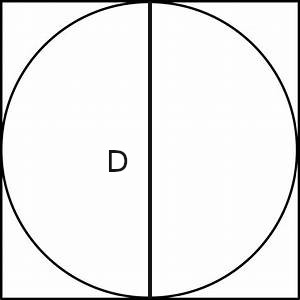
\includegraphics[width=0.3\textwidth]{figures/circle_inscribed.jpeg}
	\caption{A circle of diameter $D$ inscribed in a square.}
	\label{fig:circle_inscribed}
\end{figure}

Computing the ratio of the area of the 2 figures

\begin{equation}
\frac{\textrm{Area Circle}}{\textrm{Area Square}} = \frac{\pi D^2/4}{D^2} = \frac{\pi}{4} 
\end{equation}

The algorithm to approximate \(\pi\) should be

\begin{itemize}
\item select 2 random numbers, \(x_1\) and \(x_2\), from the interval
\([0,D]\); 
\item determine if the point defined by the ordered pair
\((x_1, x_2)\) lies within or on the circle, keeping track of the total number of
tested points and of those satisfying the condition \(D \le\sqrt{x_1^2 + x_2^2}\); 
\item approximate the ratio of the areas by the number of points within or on
the circle divided by the total number of tested points; 
\item multiply the approximated area by 4 to get \(\pi\).
\end{itemize}

\begin{codebox}[breakable, size=fbox, boxrule=1pt, pad at break*=1mm,colback=cellbackground, colframe=cellborder]
\begin{Verbatim}[commandchars=\\\{\}]
\PY{k+kn}{from} \PY{n+nn}{random} \PY{k}{import} \PY{n}{random}\PY{p}{,} \PY{n}{seed}
\PY{k+kn}{from} \PY{n+nn}{math} \PY{k}{import} \PY{n}{sqrt}
	
\PY{n}{seed}\PY{p}{(}\PY{l+m+mi}{1}\PY{p}{)}
\PY{n}{in\PYZus{}circle} \PY{o}{=} \PY{l+m+mf}{0.0}
\PY{n}{trials} \PY{o}{=} \PY{l+m+mi}{10000}
	
\PY{k}{for} \PY{n}{\PYZus{}} \PY{o+ow}{in} \PY{n+nb}{range}\PY{p}{(}\PY{n}{trials}\PY{p}{)}\PY{p}{:}
    \PY{n}{x1} \PY{o}{=} \PY{n}{random}\PY{p}{(}\PY{p}{)}
    \PY{n}{x2} \PY{o}{=} \PY{n}{random}\PY{p}{(}\PY{p}{)}
    \PY{n}{r} \PY{o}{=} \PY{n}{sqrt}\PY{p}{(}\PY{n+nb}{pow}\PY{p}{(}\PY{n}{x1}\PY{p}{,} \PY{l+m+mi}{2}\PY{p}{)} \PY{o}{+} \PY{n+nb}{pow}\PY{p}{(}\PY{n}{x2}\PY{p}{,} \PY{l+m+mi}{2}\PY{p}{)}\PY{p}{)}
    \PY{k}{if} \PY{n}{r} \PY{o}{\PYZlt{}}\PY{o}{=} \PY{l+m+mi}{1}\PY{p}{:}
        \PY{n}{in\PYZus{}circle} \PY{o}{+}\PY{o}{=} \PY{l+m+mi}{1}
	
\PY{n+nb}{print} \PY{p}{(}\PY{l+s+s2}{\PYZdq{}}\PY{l+s+s2}{Approx. pi: }\PY{l+s+si}{\PYZob{}\PYZcb{}}\PY{l+s+s2}{\PYZdq{}}\PY{o}{.}\PY{n}{format}\PY{p}{(}\PY{n}{in\PYZus{}circle}\PY{o}{/}\PY{n}{trials}\PY{o}{*}\PY{l+m+mi}{4}\PY{p}{)}\PY{p}{)}

Approx. pi: 3.1416
\end{Verbatim}
\end{codebox}

\section{Accuracy of Monte Carlo Simulation}
\label{sec:confidence_interval}

The central limit theorem~\cite{bib:central_limit} states that if we have
\(Y_1, Y_2,\dots, Y_n\) which are random samples from a distribution
\(Y\) with true mean \(\mu\) and variance \(\sigma^{2}\), then if \(n\)
is sufficiently large,

\begin{equation*} 
\mu_n = \cfrac{1}{n}\sum_i^n Y_i
\end{equation*}
 has approximately a normal distribution \(\mathcal{N}(\mu, \sigma^2/n)\).

This means that if one repeats the MC experiment many times 
(e.g. changing the seed of the random number generator) would obtain results normally distributed around the \emph{true} value \(\mu\).
We can check the central limit theorem by repeating many times the
MC experiment with our virtual deck and check how the distribution of $\mu_n$ behaves.

\begin{codebox}[breakable, size=fbox, boxrule=1pt, pad at break*=1mm,colback=cellbackground, colframe=cellborder]
\begin{Verbatim}[commandchars=\\\{\}]
\PY{c+c1}{\PYZsh{} define the domain of inputs}
\PY{k+kn}{import} \PY{n+nn}{numpy} \PY{k}{as} \PY{n+nn}{np}
\PY{k+kn}{from} \PY{n+nn}{random} \PY{k}{import} \PY{n}{sample}\PY{p}{,} \PY{n}{seed}
	
\PY{n}{deck} \PY{o}{=} \PY{p}{[}\PY{l+s+s1}{\PYZsq{}}\PY{l+s+s1}{A}\PY{l+s+s1}{\PYZsq{}}\PY{p}{,} \PY{l+s+s1}{\PYZsq{}}\PY{l+s+s1}{K}\PY{l+s+s1}{\PYZsq{}}\PY{p}{,}  \PY{l+s+s1}{\PYZsq{}}\PY{l+s+s1}{Q}\PY{l+s+s1}{\PYZsq{}}\PY{p}{,} \PY{l+s+s1}{\PYZsq{}}\PY{l+s+s1}{J}\PY{l+s+s1}{\PYZsq{}}\PY{p}{,} \PY{l+s+s1}{\PYZsq{}}\PY{l+s+s1}{2}\PY{l+s+s1}{\PYZsq{}}\PY{p}{,} \PY{l+s+s1}{\PYZsq{}}\PY{l+s+s1}{3}\PY{l+s+s1}{\PYZsq{}}\PY{p}{,} \PY{l+s+s1}{\PYZsq{}}\PY{l+s+s1}{4}\PY{l+s+s1}{\PYZsq{}}\PY{p}{,} \PY{l+s+s1}{\PYZsq{}}\PY{l+s+s1}{5}\PY{l+s+s1}{\PYZsq{}}\PY{p}{,} \PY{l+s+s1}{\PYZsq{}}\PY{l+s+s1}{6}\PY{l+s+s1}{\PYZsq{}}\PY{p}{,} \PY{l+s+s1}{\PYZsq{}}\PY{l+s+s1}{7}\PY{l+s+s1}{\PYZsq{}}\PY{p}{]} \PY{o}{*} \PY{l+m+mi}{4}
\PY{n}{experiments} \PY{o}{=} \PY{l+m+mi}{10000}
\PY{n}{trials} \PY{o}{=} \PY{l+m+mi}{10000}
\PY{n}{r} \PY{o}{=} \PY{p}{[}\PY{p}{]}
\PY{k}{for} \PY{n}{e} \PY{o+ow}{in} \PY{n+nb}{range}\PY{p}{(}\PY{n}{experiments}\PY{p}{)}\PY{p}{:}
    \PY{n}{seed}\PY{p}{(}\PY{n}{e}\PY{p}{)}
    \PY{n}{successes} \PY{o}{=} \PY{l+m+mf}{0.0}
    \PY{k}{for} \PY{n}{i} \PY{o+ow}{in} \PY{n+nb}{range}\PY{p}{(}\PY{n}{trials}\PY{p}{)}\PY{p}{:}
        \PY{n}{cards} \PY{o}{=} \PY{n}{sample}\PY{p}{(}\PY{n}{deck}\PY{p}{,} \PY{l+m+mi}{2}\PY{p}{)}
        \PY{k}{if} \PY{n}{cards} \PY{o}{==} \PY{p}{[}\PY{l+s+s1}{\PYZsq{}}\PY{l+s+s1}{K}\PY{l+s+s1}{\PYZsq{}}\PY{p}{,} \PY{l+s+s1}{\PYZsq{}}\PY{l+s+s1}{K}\PY{l+s+s1}{\PYZsq{}}\PY{p}{]}\PY{p}{:}
            \PY{n}{successes} \PY{o}{+}\PY{o}{=} \PY{l+m+mi}{1}
	
    \PY{n}{r}\PY{o}{.}\PY{n}{append}\PY{p}{(}\PY{n}{successes}\PY{o}{/}\PY{n}{trials}\PY{p}{)}
	
\PY{n+nb}{print} \PY{p}{(}\PY{l+s+s2}{\PYZdq{}}\PY{l+s+s2}{Mean: }\PY{l+s+s2}{\PYZdq{}}\PY{p}{,} \PY{n}{np}\PY{o}{.}\PY{n}{mean}\PY{p}{(}\PY{n}{r}\PY{p}{)}\PY{p}{)}
\PY{n+nb}{print} \PY{p}{(}\PY{l+s+s2}{\PYZdq{}}\PY{l+s+s2}{Std : }\PY{l+s+s2}{\PYZdq{}}\PY{p}{,} \PY{n}{np}\PY{o}{.}\PY{n}{std}\PY{p}{(}\PY{n}{r}\PY{p}{)}\PY{p}{)}

Mean:  0.00769388
Std :  0.0008770499105524154
\end{Verbatim}
\end{codebox}

Looking at Fig.~\ref{fig:repeated_MC} it is clear how increasing the number of
experiments the distribution of the results becomes more and more Gaussian-like.

\begin{figure}[htb]
	\centering
	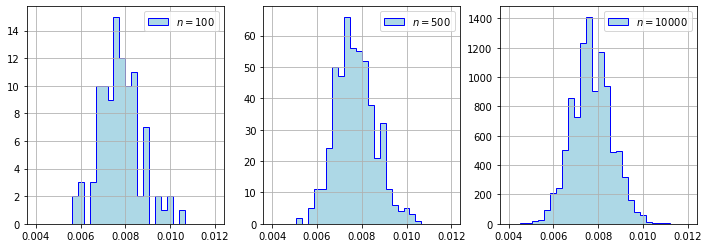
\includegraphics[width=1\textwidth]{figures/central_limit}
	\caption{Evolution of the distribution of $\mu_n$ with the increase of
	the number of MC experiments (100, 500, 10000).}
\label{fig:repeated_MC}
\end{figure}

From the central limit theorem hence: 

\begin{equation}
\mu_n - \mu \approx \mathcal{N}(0, \sigma^2/n)
\end{equation}

From the previous equation and remembering the definition of quantiles~\ref{sec:quantile-function} it is possible to define an interval so that there is a certain probability to find $\mu$ in there. Referring to Fig.~\ref{fig:confidence_interval} we can write:

\begin{equation}
P\left(\mu_n - \cfrac{1.96\sigma}{\sqrt{n}}\le \mu \le \mu_n + \cfrac{1.96\sigma}{\sqrt{n}}\right) = 0.95
\end{equation}
probability which correspond to the shaded area.

\begin{figure}[htb]
	\centering
	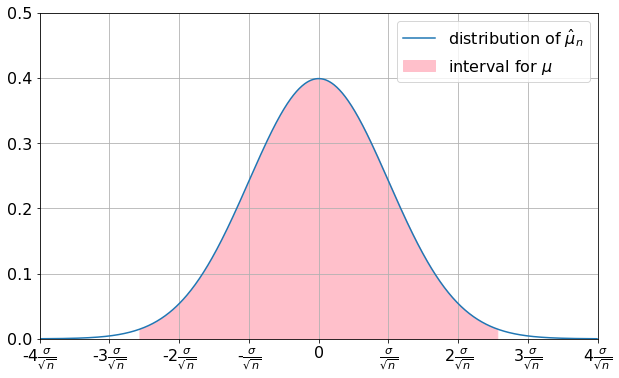
\includegraphics[width=0.7\textwidth]{figures/confidence_interval.png}
	\caption{Confidence interval for a MC experiment.}
	\label{fig:confidence_interval}
\end{figure}

This interval is called \textbf{95\% confidence interval} because
it covers 95\% of the total area under the Gaussian. It can be
interpreted like the following: if you repeat many times a simulation, 
the fraction of calculated confidence intervals that contains the true
parameter $\mu$ would tend toward 95\%.

The most commonly used intervals are 99\% and 95\% confidence level and are
respectively defined as \(\pm \cfrac{2.57\sigma}{\sqrt{n}}\) and
\(\pm \cfrac{1.96\sigma}{\sqrt{n}}\).

To construct an interval with a custom confidence level $\alpha$, we have to find a number $A$ such that
\begin{equation}
\Phi(A) = 1 - \frac{1-\alpha}{2}\quad\implies\quad A = \Phi^{-1}\left(\cfrac{1+\alpha}{2}\right)
\label{for:A}
\end{equation}
then the $\alpha$-confidence interval guarantees
\begin{equation}
P(\mu - A\sigma \le X \le \mu+ A\sigma) = \alpha 
\end{equation}

Below an example of how to compute a confidence level in \texttt{python} given a set of fake simulations. To note that the inverse of the Gaussian CDF ($\Phi^{-1}$), used in Equation~\ref{for:A}, is computed with the method \texttt{norm.ppf()} (more details on CDF in Chapter~\ref{quantile-function}).

\begin{codebox}[breakable, size=fbox, boxrule=1pt, pad at break*=1mm,colback=cellbackground, colframe=cellborder]
\begin{Verbatim}[commandchars=\\\{\}]
\PY{k+kn}{import} \PY{n+nn}{numpy} \PY{k}{as} \PY{n+nn}{np}
\PY{k+kn}{from} \PY{n+nn}{scipy}\PY{n+nn}{.}\PY{n+nn}{stats} \PY{k}{import} \PY{n}{norm}
	
\PY{n}{samples} \PY{o}{=} \PY{p}{[}\PY{l+m+mf}{1.}\PY{p}{,}\PY{l+m+mf}{2.}\PY{p}{,}\PY{l+m+mf}{3.}\PY{p}{,}\PY{l+m+mf}{4.}\PY{p}{,}\PY{l+m+mf}{4.}\PY{p}{,}\PY{l+m+mf}{4.}\PY{p}{,}\PY{l+m+mf}{5.}\PY{p}{,}\PY{l+m+mf}{5.}\PY{p}{,}\PY{l+m+mf}{5.}\PY{p}{,}\PY{l+m+mf}{5.}\PY{p}{,}\PY{l+m+mf}{4.}\PY{p}{,}\PY{l+m+mf}{4.}\PY{p}{,}\PY{l+m+mf}{4.}\PY{p}{,}\PY{l+m+mf}{6.}\PY{p}{,}\PY{l+m+mf}{7.}\PY{p}{,}\PY{l+m+mf}{8.}\PY{p}{]}
\PY{n}{alpha} \PY{o}{=} \PY{l+m+mf}{0.95}
	
\PY{n}{X} \PY{o}{=} \PY{n}{np}\PY{o}{.}\PY{n}{array}\PY{p}{(}\PY{n}{samples}\PY{p}{)}
\PY{n}{A} \PY{o}{=} \PY{n}{norm}\PY{o}{.}\PY{n}{ppf}\PY{p}{(}\PY{p}{(}\PY{l+m+mi}{1} \PY{o}{+} \PY{n}{alpha}\PY{p}{)}\PY{o}{/}\PY{l+m+mi}{2}\PY{p}{)}
\PY{n}{m}\PY{p}{,} \PY{n}{se} \PY{o}{=} \PY{n}{np}\PY{o}{.}\PY{n}{mean}\PY{p}{(}\PY{n}{X}\PY{p}{)}\PY{p}{,} \PY{n}{np}\PY{o}{.}\PY{n}{std}\PY{p}{(}\PY{n}{X}\PY{p}{)}
\PY{n}{h} \PY{o}{=} \PY{n}{A}\PY{o}{*}\PY{n}{se}\PY{o}{/}\PY{n}{np}\PY{o}{.}\PY{n}{sqrt}\PY{p}{(}\PY{n+nb}{len}\PY{p}{(}\PY{n}{samples}\PY{p}{)}\PY{p}{)}
\PY{n+nb}{print} \PY{p}{(}\PY{l+s+s2}{\PYZdq{}}\PY{l+s+si}{\PYZob{}:.0f\PYZcb{}}\PY{l+s+si}{\PYZpc{} c}\PY{l+s+s2}{onfidence interval: }\PY{l+s+si}{\PYZob{}\PYZcb{}}\PY{l+s+s2}{ +\PYZhy{} }\PY{l+s+si}{\PYZob{}\PYZcb{}}\PY{l+s+s2}{\PYZdq{}}\PY{o}{.}\PY{n}{format}\PY{p}{(}\PY{n}{alpha}\PY{o}{*}\PY{l+m+mi}{100}\PY{p}{,} \PY{n}{m}\PY{p}{,} \PY{n}{h}\PY{p}{)}\PY{p}{)}
	
95\% confidence interval: 4.4375 +- 0.8119808363806419
\end{Verbatim}
\end{codebox}

The confidence interval can be used to assess the accuracy of the Monte
Carlo simulation. From what has been said abovem the uncertainty on our best estimate of $\mu$ is $\sqrt{\cfrac{\sigma^2}{n}}=\cfrac{\sigma}{\sqrt{n}}$
where \(\sigma^2 = \mathrm{Var}(Y)\).

While it is obvious that the estimate should get worse with increased variance and better with increased sample size, this equation  gives us the exact 
scaling. Indeed the uncertainty formula tells us that to get one more decimal digit of accuracy (i.e. an error one tenth as large) requires a 100-fold increase in computation. To get three more digits of accuracy requires one million times as much computation. From that it is clear that Monte Carlo computation is poorly suited for problems that must be answered with high precision.

\begin{thebibliography}{9}
\bibitem{bib:monte_carlo}\href{https://www.youtube.com/watch?v=OgO1gpXSUzU}{\emph{Monte Carlo Simulation}}, MIT Course [Online]
\bibitem{bib:central_limit} \href{https://en.wikipedia.org/wiki/Central_limit_theorem}{\emph{Central Limit Theorem}}, Wikipedia [Online]
\bibitem{bib:confidence_interval}\href{https://www.statisticshowto.com/probability-and-statistics/confidence-interval}{\emph{Confidence Interval: How to Find a Confidence Interval: The Easy Way!}}, Statistic Howto [Online]
\end{thebibliography}









